

\chapter{Indirekte Lösungsmethoden}
\section{Theoretische Grundlagen}
Ausgangspunkt dieses Abschnittes\footnote{Hinweis: Nachfolgende Theorie orientiert sich sehr stark an \cite{NumSkript}.} ist die allgemeine Definition eines optimalen Steuerprozesses.
\begin{definition}[Optimaler Steuerprozess]{def:OptSteu}
	 Sei der zulässige Steuerbereich $U \subset \mathbb{R}^m$ nichtleer, konvex und abgeschlossen, dann ist ein allgemeiner optimaler Steuerprozess definiert als:
	\begin{align}
		\text{Minimiere } &F(x,u) = g(x(T)) + \int_0^T f_0(t,x(t),u(t)) \: dt  \\
						\text{s.t. }& \dot{x} = f(t,x,u), \quad t \in [0,T] \nonumber\\
							 				  &x(0) = x_0, \qquad \: \: \psi(x(T)) = 0 \nonumber\\
							 				  &u(t) \in U \nonumber
	\end{align}
	Dabei ist $\psi: \mathbb{R}^n \rightarrow \mathbb{R}^r$ eine $C^1$-Funktion ($0\leq r \leq n$) und $T$ die Endzeit  des Prozesses.
\end{definition}
%HAMILTONFUNKTION----------------------------------------------------------------------------------------------------------
Des Weiteren wird für den Steuerprozess \ref{def:OptSteu} die Hamilton-Funktion wie folgt definiert:
\begin{align}
	H(t,x,\lambda,u) := \lambda_0 \cdot f_0(t,x,u) + \lambda^T\cdot f(t,x,u), \quad 	\lambda_0 \in \mathbb{R}, \: \lambda \in \mathbb{R}^{n}
\end{align}
Dabei wird $\lambda$ als adjungierte Variable bezeichnet. Das \textit{Minimumsprinzip von Pontryagin} (vgl. Theorem \ref{thm:Pontryagin}) ist der zentrale Satz der Theorie optimaler Steuerprozesse und vereint die notwendigen Optimalitätsbedingungen für das Problem \ref{def:OptSteu}. Unter zusätzlichen Annahmen sind die Bedingungen sogar hinreichend (vgl. Theorem \ref{thm:HinOpt}).
%Minimumprinzip von Pontryagin----------------------------------------------------------------------------------------------------------
\begin{theo}[Minimumprinzip von Pontryagin]{thm:Pontryagin}
Es sei $(x^*,u^*): [0,T]  \rightarrow \mathbb{R}^n  \times U$ eine optimale Lösung von (\ref{def:OptSteu}), wobei die Matrix $\psi_x(x^*(T))$ vollen Rang habe. 
Dann existieren $\lambda_0 \geq 0$ und eine stetige und stückweise stetig differenzierbare Funktion $\lambda: [0,T] \rightarrow \mathbb{R}^n$ und ein Vektor $\nu \in \mathbb{R}^r$ mit $(\lambda_0, \lambda(t), \nu) \neq 0$ für alle $t \in [0,T]$, sodass die folgenden Aussagen gelten:
\begin{enumerate}
	\renewcommand{\labelenumi}{(\roman{enumi})}
	\item An allen Stetigkeitsstellen $t \in [0,T]$ von $u^*(\cdot)$ gilt die Minimumsbedingung
		\begin{align}
			H(t,x^*(t),\lambda(t),u^*(t)) = \min_{u \in U} 	H(t,x^*(t),\lambda(t),u) 
			\label{eqn:Minimumsbedingung}
		\end{align}
	\item An allen Stetigkeitsstellen $t \in [0,T]$ von $u^*(\cdot)$ gilt die adjungierte Differentialgleichung
		\begin{align}
			\dot{\lambda}(t)^T = -H_x(t,x^*(t),\lambda(t),u^*(t))
		\end{align}
	\item Im Endzeitpunkt $T$ gilt die Transversalitätsbedingung
		\begin{align}
			\lambda(T)^T = \lambda_0g_x(x^*(T))+\nu^T\psi_x(x^*(T))
		\end{align}
	\item Im Falle freier Endzeit gilt für die optimale Endzeit $T^*$
		\begin{align}
			H(T^*,x^*(T^*),\lambda(T^*),u^*(T^*)) = 0 
		\end{align}
	\item Für autonome Systeme gilt außerdem
		\begin{align}
			H(T^*,x^*(T^*),\lambda(T^*),u^*(T^*)) = \text{const in } [0,T]
		\end{align}
\end{enumerate}
\end{theo}
\pagebreak

Korollar \ref{kor:FreierEndzustand} ergänzt für eine wichtige Modellklasse (freier Endzustand) die Aussage von Theorem \ref{thm:Pontryagin}.
\begin{korollar}[]{kor:FreierEndzustand}
	Bei freiem Endzustand $x(T)$, d.h., im Falle $\psi \equiv 0$, kann ohne Beschränkung der Allgemeinheit $\lambda_0 = 1$ in Theorem \ref{thm:Pontryagin} angenommen werden.
\end{korollar}

\begin{theo}[Hinreichende Optimalitätsbed. für opt. Steuerprozesse]{thm:HinOpt}
	Es sei $(x^*,u^*)$ ein zulässiges Paar für das Problem \ref{def:OptSteu}. Es existieren eine Funktion $\lambda:[0,T] \rightarrow \mathbb{R}^n$ und ein $\nu \in \mathbb{R}^r$, sodass die Bedingungen von Satz \ref{thm:Pontryagin} mit $\lambda_0 = 1$ erfüllt sind. Zusätzlich sei
	\begin{itemize}
		\item[(a)] $\psi(\cdot)$ affin-linear \label{item:HinOptA}
		\item[(b)] $g(\cdot)$ konvex und \label{item:HinOptB}
		\item[(c)] $H^{(0)}:= \min_{u \in U} H(t,x,\lambda,u)$ konvex in x für jedes $(t,\lambda(t))$.\label{item:HinOptC}
	\end{itemize}
	Damit ist $(x^*,u^*)$ eine optimale Lösung des Problems \ref{def:OptSteu}.
\end{theo}

Damit sichergestellt werden kann, ob das Minimumsprinzip von Pontryagin anwendbar ist, ist die Steuerfunktion $u(t)$ auf Stetigkeit zu überprüfen. Zu diesem Zweck wird ein Regularitätsbegriff bezogen auf die Hamilton-Funktion (vgl. Definition \ref{def:Reularität}) eingeführt, welcher unter gewissen Umständen Stetigkeit garantiert (vgl. Korollar \ref{kor:StetigkeitRegularität}).

\begin{definition}[Regularität der Hamilton-Funktion]{def:Reularität}
	Die Hamilton-Funktion $H(t,x,\lambda,u)$ heißt regulär (bzgl. einer optimalen Lösung $x^*(t), \lambda^*(t)$), wenn es ein $\epsilon > 0$ gibt, sodass für die Menge
	\begin{align*}
	D_\epsilon = \{(t,x,\lambda):t \in [0,T], || x - x^*(t) || < \epsilon, || \lambda - \lambda^*(t) || < \epsilon \}
	\end{align*}
	gilt: Die Hamilton-Funktion hat eine eindeutig bestimmte Minimalstelle
	\begin{align*}
	u^*(t,x,\lambda) = \operatorname{arg} \min\limits_{u\in U} H(t,x,\lambda,u) \text{ } \forall \text{ } (t,x,\lambda) \in D_\epsilon.
	\end{align*}
\end{definition}

\begin{korollar}[]{kor:StetigkeitRegularität}
Im Falle einer regulären Hamilton-Funktion ist die optimale Steuerung $u^*(t)$ stetig. Ist $U=\mathbb{R}^m$, so ist die optimale Steuerung $u^*(t)$ sogar eine $C^k$-Funktion ist.
\end{korollar}
%\subsection{Leitfaden}
%\begin{enumerate}
%	\item Pontryagin anwendbar? -> Stetigkeit von u muss gesichert sein, weil Pontryagin nur an Stetigkeitsstellen gilt
%	\item Stetigkeitsüberprüfung über Regularität der Hamilton-Funktion
%	\item  Wenn Hamilton-Funktion eindeutiges Minimum besitzt => Hamilton-Funktion regulär und u stetig
%	\begin{itemize}
%		\item Stetiger  Differenzierbarkeit der Hamilton-Funktion nachweisen
%		\item 1. und 2. Ableitung der Hamilton-Funktion betrachten
%	\end{itemize}
%	\item Optimale Steuerung über Fallunterscheidung herleiten
%	\item Randwertproblem aufstellen
%	\item verschiedene Algorithmen ausprobieren
%\end{enumerate}

%Notizen:
%\begin{itemize}
%	\item \textbf{keine} freie Endzeit, $T=1$
%	\item freier Endzustand $\psi(x(T)) \equiv  0 \rightarrow \lambda_0 = 1$ nach Korollar \ref{kor:FreierEndzustand} 
%	\item Steuerbeschränkungen $u \in [0,5]$
%	\item Startwert $x_0 = [1, 0]^T$
%	\item autonomes Problem
%	\item Mayer-Problem
%	\item Steuerfunktion $u$ geht nichtlinear ein
%\end{itemize}

\section{Problemanalyse} \label{sec:Problemanalyse}

Wird das Problem aus \autoref{ch:Aufgabe} näher betrachtet fällt auf, dass keine variable Endzeit vorliegt ($T=1$). Des Weiteren ist Korollar \ref{kor:FreierEndzustand} anwendbar, da der Endzustand  frei ist ($\psi(x(T) \equiv  0 $), wodurch in der Hamilton-Funktion $\lambda_0 = 1$  angenommen werden darf. Die Steuerung $u:= u(t)$ muss sich im Bereich $U = [0,5]$ bewegen und geht nichtlinear in die Dynamik ein. Durch die fehlende direkte Zeitabhängigkeit des Differentialgleichungssystems liegt ein autonomes System in Zusammenspiel mit einem reinen Mayer-Problem vor. Demnach folgt aus der Zustandsbeschreibung:

\begin{align*}
	f_0(t,x(t),u(t))  &\equiv 0 	&\text{(LagrangeTerm)}\\
	g(x(T)) &= -x_2(T) &\text{(Mayer-Term)}\\
	f (t,x(t),u(t))		&= \left(\begin{array}{c} 		-ux_1(t)+u^2x_2(t)\\ 
																ux_1(t) - 3u^2x_2(t) \end{array}\right)&\text{(DGL-System)}
\end{align*}
		
Entsprechend dem Minimumprinzip von Pontryagin (Theorem \ref{thm:Pontryagin}) ist aus den erlangten Erkenntnissen die problemspezifische Hamilton-Funktion,						
\begin{align}
	H(t,x(t),\lambda(t),u(t)) &=  \underbrace{\lambda_0  \cdot f_0(t,x,u)}_{=0}+ \lambda^T\cdot f(t,x,u)\\
										 %&= \lambda_1(t) \cdot  \left[ -ux_1(t)+u^2x_2(t)\right] +  \lambda_2(t) \cdot  \left[ ux_1(t) - 3u^2x_2(t) \right]\\
										 %&=  - \lambda_1(t) x_1(t) u+  \lambda_1(t) x_2(t)u^2  +  \lambda_2(t) x_1(t)u -  3 \lambda_2(t) x_2(t)u^2
										 &=  (- \lambda_1(t) +  \lambda_2(t))\cdot x_1(t) u + (\lambda_1(t) -  3 \lambda_2(t)) \cdot  x_2(t)u^2
\end{align}

die adjungierte Differentialgleichung 
\begin{align}
	\dot{\lambda}(t)^T	&= - H_x(t,x^*(t),\lambda(t),u^*(t))\\
%												&=- \left(\begin{array}{c} 	 - \lambda_1(t) u  + \lambda_2(t) u\\
%																											 \lambda_1(t) u^2 -  3 \lambda_2 (t)u^2 \end{array}\right)\\
											    &= \left(\begin{array}{c} 	 \lambda_1(t) u  - \lambda_2(t) u\\
																			 								-\lambda_1(t) u^2  + 3 \lambda_2(t) u^2 \end{array}\right)
\end{align}
und die Transversalitätsbedingung
\begin{align}
	\lambda(T)^T = \underbrace{\lambda_0}_{=1 \text{ (Korollar \ref{kor:FreierEndzustand})}}g_x(x^*(T))+\underbrace{\nu^T\psi_x(x^*(T))}_{=0, \text{ da } \psi \equiv  0} \overset{!}{=}  \left(\begin{array}{c} 0\\-1\end{array}\right)
\end{align}
ableitbar. Da zusätzlich ein autonomes System vorliegt, ist die Hamilton-Funktion konstant für alle $t \in [0,T]$ und es gilt:
\begin{align}
	H(x^*(t),\lambda(t), u^*(t)) = c = \text{ konstant in } [0,1]
\end{align}

\section{Stetigkeitsüberprüfung der Steuerfunktion} \label{sec:Stetigkeit}
Zur Anwendung der Minimumsbedingung (\ref{eqn:Minimumsbedingung}) des Pontryagischen Minimumsprinzips (vgl. Theorem \ref{thm:Pontryagin}) muss zunächst die Stetigkeit der optimalen Steuerfunktion $u^*(t)$ auf dem gesamten betrachteten Zeitintervall sichergestellt werden.
Dies kann anhand einer Regularitätsuntersuchung der Hamilton-Funktion erfolgen. Dazu belegen wir in diesem Abschnitt zunächst die partielle, stetige Differenzierbarkeit der Hamilton-Funktion nach der Steuerung $u$, als Vorraussetzung für die nachfolgende Regularitätsanalyse.  
%Als Vorraussetzung für eine Regularitätsanalyse stellen wir in diesem Abschnitt zunächst partiell stetige Differenzierbarkeit der Hamilton-Funktion nach der Steuerung $u$ 
%Alt:
%Dazu wird in diesem Abschnitt zunächst die partiell stetige Differenzierbarkeit der Hamilton-Funktion nach der Steuerung $u$, als Voraussetzung für eine Regularitätsanalyse sichergestellt. Im Anschluss untersuchen wir die Hamilton-Funktion hinsichtlich Ihrer Regularitätsbedingung, da diese die Stetigkeit der Optimalsteuerung sicherstellt. 
%%%
%Da bei regulärer Hamilton-Funktion die optimale Steuerung stetig ist, untersuchen wir zunächst die Regularitätsbedingung der Hamilton-Funktion. 
%%%
%Dazu wird in diesem Abschnitt zunächst hinsichtlich Ihrer Regularitätseigenschaft untersucht, da bei regulärer Hamilton-Funktion die optimale Steuerung stetig ist. Als 
%%%
%Dazu wird in diesem Abschnitt zunächst die partiell stetige differenzierbarkeit der Hamilton-Funktion nachgewiesen. Anschließend untersuchen wir die Hamilton-Funktion hinsichtlich ihrer Regularitätseigenschaft, die einhergeht mit einer stetigen Steuerfunktion. 
\subsection{Stetige Differenzierbarkeit der Hamilton-Funktion}
Ziel ist es, die zweifache partielle stetige Differenzierbarkeit der Hamilton-Funktion nach der Steuerfunktion $u$ im gesamten Zeitintervall $[0,1]$ nachzuweisen. 
Dazu sei $t \in [0,1]$ beliebig aber fest mit zugehörigem $x:=x(t)$ und $\lambda:=\lambda(t)$. Die Hamilton-Funktion lässt sich dann, zu einem festen Zeitpunkt, als Funktion der Steuerung $u$ mit Definitionsbereicht $U$ interpretieren:
\begin{align}
	H: U \rightarrow \mathbb{R}, u \mapsto H(u) = (-\lambda_1 + \lambda_2) \cdot x_1 \cdot u + (\lambda_1 - 3 \lambda_2) \cdot x_2 \cdot u^2.
	\label{eqn:H(u)}
\end{align} 
Es ist erkennbar, dass es sich bei $H(u)$ um ein Polynom zweiten Grades handelt. Da Polynome zu den beliebig oft stetig differenzierbaren Funktionen zählen, folgt entsprechend für $H(u)$ zweifach stetige Differenzierbarkeit. Alternativ findet sich im Anhang ein ausführlicher Beweis mittels Differentialquotient und Epsilon-Delta-Kriterium (vgl. \autoref{chap:A2}). Insgesamt ergibt sich also für die Hamilton-Funktion $H(t,x,\lambda,u)$ zweifach partielle stetige Differenzierbarkeit nach $u$, für alle $t \in [0,1]$ und $u \in U$. 
\subsection{Regularitätsuntersuchung der Hamilton-Funktion}
Die Regularitätsuntersuchung der Hamilton-Funktion ist essentiell, da diese die Stetigkeit der optimalen Steuerung sicherstellt und somit eine Anwendung der Minimumsbedingung (\ref{eqn:Minimumsbedingung}) ermöglicht. Die Hamilton-Funktion heißt regulär, wenn sie zu jedem festen Zeitpunkt $t\in [0,1]$, für alle Ausprägungen $x$ und $\lambda$ aus Trajektorien $x(t)$ und $\lambda(t)$, welche innerhalb einer $\epsilon$-Umgebung um die optimalen Trajektorien $x^*(t)$ und $\lambda^*(t)$ variieren, ein eindeutiges Minimum über $u$ besitzt. \\
Es ist also in jedem Zeitschritt zu überprüfen, ob das beschränkte Optimierungsproblem
\begin{align}
	\min\limits_{u \in U} H(x(t),\lambda(t),u), \: t \in [0,T] \label{eq:min_regularität}
\end{align}
eine eindeutige Lösung besitzt. \\
%Es ist also in jedem Zeitschritt zu überprüfen, ob das beschränkte Optimierungsproblem eine eindeutige Lösung besitzt:
%\begin{align}
%	\exists! u^* = arg\min\limits_{u \in U} H(x,\lambda,u)
%\end{align}
Dazu sei im folgenden $t \in [0,1]$ beliebig, aber fest, mit zugehörigen $x := x(t)$ beliebig, aber fest und $\lambda := \lambda(t)$ beliebig, aber fest, sowie $u := u(t) \in U$. 
%Im folgenden seien:
%\begin{align}
%	&t \in [0,1] \text{ beliebig aber fest mit zugehörigen Trajektorien} \nonumber \\
%	&\lambda := \lambda(t) \text{ beliebig aber fest} \nonumber \\
%	&x := x(t) \text{ beliebig aber fest}
%\end{align}
Da es sich als physikalisch sinnvoll erweist positive Konzentrationen zu betrachten, gelte für die Stoffkonzentrationen im Weiteren stets:
\begin{align}
	& x_1(t) > 0 \text{ } \forall \text{ } t \in [0,1], \nonumber \\
	& x_2(t) > 0 \text{ } \forall \text{ } t \in (0,1]. \label{eq:annahme_x_pos}
\end{align}
Außerdem ist zu beachten, dass die untere Steuerintervallgrenze $u_{min} = 0$ widersprüchlich zum exponentiellen Zusammenhang (\ref{eq:k1}) zwischen transformierter Steuervariable $u(t)$ und ortsabhängiger Reaktortemperatur $\theta(t)$ ist. Die Steuerung $u$ sollte deshalb, soweit möglich, nicht die untere Steuerintervallgrenze $u_{min}$ annehmen. \\
 Im folgenden betrachten wir das vorliegende Optimierungsproblem (\ref{eq:min_regularität}) zunächst mit unbeschränktem Steuerintervall $U = \mathbb{R}$, hinsichtlich möglicher Extremwerte und ziehen anhand dessen Rückschlüsse über das Auftreten von Minima $u^*$ im beschränkten Fall, mit $U=[0,5]$. \\
%Dazu betrachten wir das Problem im folgenden zunächst als unbeschränktes Optimierungsproblem mit $U = \mathbb{R}$ und ziehen dann Rückschlüsse auf das beschränkte  
%Es ist hilfreich die Hamilton-Funktion, wie bereits in (\ref{eqn:H(u)}), zu einem festen Zeitpunkt $t \in [0,1]$ wieder als Funktion $H(u)$ über der Steuerung $u \in U$ mit festem $x:=x(t)$ und $\lambda:=\lambda(t)$ aufzufassen:
%\begin{align}
%	H: U \rightarrow \mathbb{R}, u \mapsto H(u) = (-\lambda_1 + \lambda_2) \cdot x_1 u + (\lambda_1 - 3 \lambda_2) \cdot x_2 u^2
%\end{align} 
%\\
Im unbeschränkten Fall lautet das notwendige Kriterium für lokale Extrema:
\begin{align}
	&H_u(x,\lambda,u)  =  (-\lambda_1 + \lambda_2) \cdot x_1 + 2 \cdot (\lambda_1 - 3 \lambda_2) \cdot x_2 \cdot u = 0. \label{eq:NotwBedExtrema}
\end{align}
Durch umstellen ergibt sich bei
\begin{align}
	&\overline{u}  :=  \frac{(\lambda_1-\lambda_2) \cdot  x_1}{(2 \lambda_1 -  6 \lambda_2) \cdot  x_2} 
	\label{eq:Extremstelle}
\end{align}
die einzige, eindeutige Extremstelle, wobei $(2 \lambda_1 -  6 \lambda_2) \neq  0$ und $x_2 \neq  0$ gelten muss. Die Art der Extremstelle lässt sich anhand des Vorzeichens der zweiten partiellen Ableitung
\begin{align}
	&H_{uu}(x,\lambda,u)  = (2 \lambda_1 -  6 \lambda_2) \cdot  x_2
\end{align}
charakterisieren. \\
Es ergeben sich die folgenden drei Fälle zur näheren Betrachtung:
\subsubsection*{Fall 1: \boldmath$\lambda_1 > 3\lambda_2 \land x_2 > 0$}
Falls $\lambda_1 > 3\lambda_2$ und $x_2 > 0$, so gilt für die zweite Ableitung an der Extremstelle
\begin{align}
	&H_{uu}(x, \lambda, \overline{u})  = (2 \lambda_1 -  6 \lambda_2) \cdot  x_2 > 0.
\end{align}
Somit erfüllt $\overline{u}$ die hinreichende Bedingung für eine Minimalstelle und die Hamilton-Funktion besitzt im unbeschränkten Fall $U = \mathbb{R}$ ein eindeutiges Minimum über $u$. Da mit $\overline{u}$ lediglich eine eindeutige Extremstelle in Form eines Minimums auftritt, lässt sich daraus folgern, dass die Hamilton-Funktion links von dieser streng monoton fallend und rechts davon, streng monoton steigend, über $u$, verlaufen muss. \\ 
Wird nun der beschränkte Fall $U = [0,5]$ betrachtet, so ergeben sich für ein potentielles Minimum $u^*$ drei mögliche Teilfälle: 
\begin{enumerate}[label=(\alph*)]
	\item Das Minimum des unbeschränkten Problems liegt innerhalb der Steuerbeschränkung. Das eindeutige Minimum des beschränkten Problems entspricht folglich dem des unbeschränkten Problems: \\
$\overline{u} \in U = [0,5] \Rightarrow u^* = \overline{u}$
	\item Das Minimum des unbeschränkten Problems unterschreitet die Steuerbeschränkung. Das eindeutige Minimum des beschränkten Problems liegt folglich auf der unteren Steuerintervallgrenze:\\
$\overline{u} < u_{min} = 0 \Rightarrow u^* = u_{min} = 0$
	\item Das eindeutige Minimum des unbeschränkten Problems überschreitet die Steuerbeschränkung. Das eindeutige Minimum des beschränkten Problems liegt folglich auf der oberen Steuerintervallgrenze: \\ 
$\overline{u} > u_{max} = 5 \Rightarrow u^* = u_{max} = 5$
\end{enumerate}
In allen Teilfällen weist das beschränkte Steuerproblem ein eindeutiges Minimum auf und die Hamilton-Funktion ist somit regulär.

\subsubsection*{Fall 2: \boldmath$\lambda_1 < 3\lambda_2 \land x_2 > 0$}
Ist $\lambda_1 < 3\lambda_2$ und $x_2 > 0$ so liegt in $\overline{u}$ ein eindeutiges Maximum vor, da für die zweite Ableitung 
\begin{align}
	&H_{uu}(x,\lambda,\overline{u})  = (2 \lambda_1 -  6 \lambda_2) \cdot  x_2(t) < 0
\end{align} gilt. 
Da $\overline{u}$ bei unbeschränktem Steuerintervall $U=\mathbb{R}$ das einzige Extremum in Gestalt eines Maximums ist, erkennt man leicht, dass die Hamilton-Funktion links davon streng monoton steigend und rechts streng monoton fallend, über $u$, verlaufen muss. 
%Da $\overline{u}$ bei unbeschränktem Steuerintervall $U=\mathbb{R}$ das einzige Extremum in Gestalt eines Maximums ist, verläuft die Hamilton-Funktion folglich links von $\overline{u}$ sterng monoton steigend und rechts von $\overline{u}$ streng monoton fallend. 
%Da lediglich eine Extremstelle bei unbeschränktem Steuerintervall auftritt, ergibt sich, ähnlich wie im vorherigen Fall, dass die Hamilton-Funktion links davon streng monoton steigend und rechts streng monoton fallend verlaufen muss. 
Für das Minimierungsproblem (\ref{eq:min_regularität}) mit beschränkten Steuerbereich $U=[0,5]$, lassen sich dann wieder mehrere Teilfälle unterscheiden:
%Bei Betrachtung des beschränkten Steuerbereichs, lassen sich dann wieder mehrere Fälle unterscheiden: 
\begin{enumerate}[label=(\alph*)]
	\item Das Maximum des unbeschränkten Problems unterschreitet die Steuerbeschränkung. Das eindeutige Minimum des beschränkten Problems liegt folglich auf der oberen Steuerintervallgrenze: \\ 
$\overline{u} < u_{min} = 0 \Rightarrow u^* = u_{max} = 5$ \label{item:Fall2a}
	\item Das Maximum des unbeschränkten Problems überschreitet die Steuerbeschränkung. Das eindeutige Minimum des beschränkten Problems liegt folglich auf der unteren Steuerintervallgrenze: \\ 
$\overline{u} > u_{max} = 5 \Rightarrow u^* = u_{min} = 0$ \label{item:Fall2b}
	\item Das Maximum des unbeschränkten Problems liegt innerhalb der Steuerbeschränkung. Es ergeben sich die möglichen Teilfälle: \label{item:Fall2c}
	\begin{enumerate}[label=(\roman*)]
		\item Das eindeutige Minimum des beschränkten Problems liegt auf der unteren Steuerintervallgrenze: \\
$u^* = u_{min} = 0 \Leftrightarrow H(u_{min}) < H(u_{max}) $ \label{item:Fall2ci}
		\item Das eindeutige Minimum des beschränkten Problems liegt auf der oberen Steuerintervallgrenze: \\
$u^* = u_{max} = 5 \Leftrightarrow H(u_{min}) > H(u_{max}) $ \label{item:Fall2cii}
		\item Es liegt kein eindeutiges Minimum vor. Die Hamilton-Funktion weißt auf den Steuerintervallgrenzen den selben Wert auf: \\
$u^* = \{u_{min}, u_{max}\} \Leftrightarrow H(u_{min}) = H(u_{max}) $ \label{item:Fall2ciii}
	\end{enumerate}
\end{enumerate}
In den Teilfällen \ref{item:Fall2a}, \ref{item:Fall2b}, \hyperref[item:Fall2c]{(c, i)}, sowie \hyperref[item:Fall2c]{(c, ii)} findet sich ein eindeutiges Minimum für die Hamilton-Funktion, womit auch deren Regularität sichergestellt ist. Problematisch ist der Teilfall \hyperref[item:Fall2c]{(c, iii)}, da bei diesem kein eindeutiges Minimum der Hamilton-Funktion gefunden werden kann. \\
Im folgenden untersuchen wir, unter welchen Bedingungen dieser Fall ausschließbar ist. Die Hamilton-Funktion nimmt an der unteren Steuerintervallgrenze $u_{min}=0$ mit
\begin{align}
	H(x,\lambda,u_{min}) = (-\lambda_1 + \lambda_2) \cdot u_{min} \cdot x_1 + (\lambda_1 - 3\lambda_2) \cdot u_{min}^2 \cdot x_2 = 0
\end{align}
stets einen konstanten Wert an. Da die untere Steuerintervallgrenze $u_{min} = 0$ widersprüchlich zum exponentiellen Zusammenhang in (\ref{eq:k1}) ist, soll das Minimum im beschränkten Fall an der oberen Steuerintervallgrenze $u_{max} = 5$ angenommen werden. Für die Hamilton-Funktion muss also
%Soll das Minimum im beschränkten Fall auf der oberen Steuerintervallgrenze liegen, so muss dort für die Hamilton-Funktion
\begin{align}
	& H(u_{max}) = H(5) \overset{!}{<} H(u_{min}) = 0 \nonumber \\
	& \Leftrightarrow (-\lambda_1 + \lambda_2) \cdot u_{max} \cdot x_1 + (\lambda_1 - 3\lambda_2) \cdot u_{max}^2 \cdot x_2 \overset{!}{<} 0 
\end{align}
gelten. Weiter ist im aktuellen Fall $\lambda_1 < 3\lambda_2$ und $x_2 > 0$, sowie wegen Annahme (\ref{eq:annahme_x_pos}) die Konzentration $x_1 > 0$, wodurch sich der Ausdruck weiter vereinfacht zu:
%Mit $\lambda_1 < 3\lambda_2$ im aktuellen Fall und der Annahme positiver Konzentrationen, also $x_1 > 0$ und $x_2 > 0$, vereinfacht sich der Ausdruck weiter zu:
\begin{align}
	&5 \cdot (-\lambda_1 + \lambda_2) \cdot \underbrace{x_1}_{>0} + 25 \cdot \underbrace{(\lambda_1 - 3\lambda_2)}_{<0}  \cdot \underbrace{x_2}_{>0} \overset{!}{<} 0. \label{eq:anforderung_Humax<Humin}
\end{align}
Da $x_2>0$ einhergeht mit Zeitpunkten $t>0$ fordert man für die adjungierte Variable
\begin{align}
	\lambda_1(t) > \lambda_2(t) \text{ } \forall \text{ } t>0 
	\label{eq:anforderung_lambda2<lambda1_t>0}
\end{align}
um die Abschätzung (\ref{eq:anforderung_Humax<Humin}) zu erfüllen. Es gilt dann
\begin{align}
\lambda_2 < \lambda_1 < 3\lambda_2 
\Leftrightarrow H(u_{max}) < H(u_{min}) 
\Leftrightarrow u^* = u_{max}.
\end{align}
%
Somit wird ein eindeutiges Minimum auf der oberen Steuerintervallgrenze $u_{max} = 5$ angenommen. Folglich kann Teilfall \hyperref[item:Fall2c]{(c, iii)} sicher ausgeschlossen werden und die Regularität ist sichergestellt.

%und die Regularität ist sichergestellt. 
\subsubsection*{Fall 3: \boldmath$x_2 = 0 \lor \lambda_1 = 3\lambda_2$}
Für $x_2 = 0$ oder $\lambda_1 = 3\lambda_2$ lässt sich nach (\ref{eq:NotwBedExtrema}) keine Extremstelle für das unbeschränkte Steuerproblem, mit $U=\mathbb{R}$, finden. Deshalb betrachten wir direkt das beschränkte Steuerproblem mit $U=[0,5]$. Die Hamilton-Funktion vereinfacht sich nun zu
\begin{align}
	H(x,\lambda, u) = (-\lambda_1 + \lambda_2) \cdot u \cdot x_1 + \underbrace{(\lambda_1 - 3\lambda_2) \cdot u^2 \cdot x_2}_{=0}
	= (-\lambda_1 + \lambda_2) \cdot u \cdot x_1
\end{align}
während für die Schaltfunktion 
\begin{align}
	H_u(x,\lambda) = (-\lambda_1 + \lambda_2) \cdot \underbrace{x_1}_{>0}
\end{align}
gilt. Dabei ist zu beachten, dass die Schaltfunktion unabhängig von $u$ ist und somit zu einem festen Zeitpunkt über dem gesamten Steuerintervall einen konstanten Wert annimmt. Außerdem gilt nach Annahme (\ref{eq:annahme_x_pos}) wieder $x_1 >0$.\\
Nach dem Satz vom Minimum und Maximum nimmt die Hamilton-Funktion im kompakten und beschränkten Steuerintervall stets ein Minimum an. Verläuft die Hamilton-Funktion streng monoton auf dem gesamten Steuerintervall, so lässt sich zusätzlich auf ein eindeutiges Minimum auf einer der beiden Intervallgrenzen schließen. \\
%streng monotonem Verlauf der Hamilton-Funktion auf dem gesamten Steuerintervall lässt sich auf ein eindeutiges Minimum schließen auf einer der Intervallgrenzen. \\
Anhand des Vorzeichens der Schaltfunktion lässt sich nun untersuchen, ob die Hamilton-Funktion einen streng monotonen Verlauf aufweist. Es ergeben sich drei mögliche Teilfälle:\
%Weißt die Schaltfunktion ein Vorzeichen ungleich Null auf, so ergibt sich für die Hamilton-Funktion ein streng monotoner Verlauf über dem gesamten Steuerintervall. Entsprechend wird auf einer der Intervallgrenzen ein eindeutiges Minimum angenommen. Andernfalls wird kein eindeutiges \\
\begin{enumerate}[label=(\alph*)]
	\item eindeutiges Minimum auf der unteren Intervallgrenze: \\
	$\lambda_1 > \lambda_2 \Leftrightarrow H_u < 0 \Leftrightarrow H \text{ streng monton fallend} \Leftrightarrow u^* = u_{max}$  \label{item:3b}
	\item eindeutiges Minimum auf der oberen Intervallgrenze: \\
	$\lambda_1 < \lambda_2 \Leftrightarrow H_u > 0 \Leftrightarrow H \text{ streng monton steigend} \Leftrightarrow u^* = u_{min}$ \label{item:3c}
	\item kein eindeutiges Minimum: \\
	$\lambda_1 = \lambda_2 \Leftrightarrow H_u = 0$ \label{item:3a}
\end{enumerate}
In den Teilfällen \ref{item:3b} und \ref{item:3c} wird ein eindeutiges Minimum angenommen und die Hamilton-Funktion ist entsprechend regulär. Der kritische Teilfall \ref{item:3a} ist für Zeitpunkte $t>0$ widersprüchlich zu Annahme (\ref{eq:anforderung_lambda2<lambda1_t>0}) und lässt sich somit auf den Zeitpunkt $t=0$ mit Startkonzentration $x_2 = 0$ zurückführen. \\
%%%%%
%In den Teilfällen \ref{item:3b} und \ref{item:3c} wird ein eindeutiges Minimum angenommen und die Hamilton-Funktion ist entsprechend regulär. Der kritische Teilfall \ref{item:3a} ist widersprüchlich zu $\lambda_1 = 3\lambda_2$ im aktuellen Fall und tritt folglich lediglich bei $x_2 = 0$ auf. Mit Annahme (\ref{eq:annahme_x_pos}) gilt außerdem $x_2>0$ $\forall$ $t>0$, wodurch sich der Teilfall \ref{item:3a} auf den Zeitpunkt $t=0$ mit $\lambda_1 = \lambda_2$ zurückführen lässt. 
%%%%%
Um auch im Startpunkt die Regularität der Hamilton-Funktion sicherzustellen, gelte bei $t=0$ als weitere Annahme 
\begin{align}
\lambda_1(0) \neq \lambda_2(0). 
\end{align} 
Soll zusätzlich sichergestellt werden, dass das Minimum auf der oberen Intervallgrenze $u_{max} = 5$ angenommen wird, gelte sogar
\begin{align}
\lambda_1(0) > \lambda_2(0). \label{eq:anforderung_lambda1>lambda2_t=0}
\end{align}
Dabei ist zu beachten, dass diese Anforderung als eine Erweiterung von Annahme (\ref{eq:anforderung_lambda2<lambda1_t>0}) im Zeitpunkt $t=0$ gesehen werden kann. 

%Wir möchten nun wieder ein Kriterium finden, so dass ein eindeutiges Minimum auf der oberen Steuerintervallgrenze $u_{max}$ eingenommen werden. Dies können wir erreichen, indem wir sicher stellen, dass die Schaltfunktion stets negative Werte annimmt. \\
%Man erkennt direkt, dass unter der Annahme $\lambda_1 > \lambda_2$, die Schaltfunktion immer negative Werte aufweist: 
%\begin{align}
%	H_u(0,x,\lambda, u) = \underbrace{(-\lambda_1 + \lambda_2)}_{<0} \cdot \underbrace{x_1}_{>0}  < 0
%\end{align}
%Die Hamilton-Funktion verläuft dann im gesamten Steuerintervall streng monoton steigend und nimmt ihr eindeutiges Minimum bei:
%\begin{align}
%	u^* = u_{max}
%\end{align}
%an. 
%

%%\begin{itemize}
%%	\item Was passiert bei $t=0$, da  dort $x_2(0) = 0 $, somit bereits gefundenes $u$ nicht definiert und $u^* \overset{!}{>} 0$. Intuitiver Ansatz es einfach auf $u_{min}=0$ zu setzen funktioniert nicht!
%%	\item Was passiert mit Bedingung an $\lambda \rightarrow$ von $H_{uu}$? 
%%	\item Fallunterscheidung auf $t$ zurückführen
%%	\item Hinweise Jörn
%%\end{itemize}
%\subsection{Untersuchung $U=\mathbb{R}$}
%Da Steuerung $u$ nichtlinear und mit Beschränkungen in die Hamilton-Funktion eingeht, ist im ersten Schritt die Hamilton-Funktion auf Regularität zu überprüfen. Zu diesem Zweck wird die Steuerbeschränkung zunächst vernachlässigt: 
%\begin{align}
%	&H_u(x,\lambda,u)  =  - \lambda_1  x_1(t)+  2 \lambda_1 u x_2(t)  +  \lambda_2  x_1(t) -  6 \lambda_2  u x_2(t) = 0\\
%	&\Leftrightarrow \lambda_2  x_1(t)  - \lambda_1  x_1(t)+ ( 2 \lambda_1 x_2(t) -  6 \lambda_2  x_2(t) ) \cdot u  = 0\\[10pt]
%	&\text{Eindeutig nach u auflösbar, somit gibt es einen eindeutigen Extrempunkt:}\nonumber\\[10pt]
%	&\Leftrightarrow  u  = \frac{\lambda_1  x_1(t)-\lambda_2  x_1(t)}{2 \lambda_1 x_2(t) -  6 \lambda_2  x_2(t)}= \frac{(\lambda_1-\lambda_2) \cdot  x_1(t)}{(2 \lambda_1 -  6 \lambda_2) \cdot  x_2(t)} \label{eq:Steuerfunktion}
%\end{align}
%Dabei muss gelten:
%\begin{align}
%	(2 \lambda_1 -  6 \lambda_2) \cdot  x_2(t) \neq  0
%\end{align}
%Dies ergibt Sinn, da $x_2(T)$ zu maximieren ist und als Konzentration des Stoffes $A_2$ immer größer als $0$ sein sollte. Überprüfung, ob Extremstelle ein Minimum ist:
%\begin{align}
%	&H_{uu}(x,\lambda,u)  = (2 \lambda_1 -  6 \lambda_2) \cdot  x_2(t) \overset{!}{>} 0
%\end{align}
%Da $x_2(t) > 0, t \in (0,1]$ muss für eine eindeutige Minimalstelle $2 \lambda_1 -  6 \lambda_2 > 0$ sein, d.h. $\lambda_1 > 3\lambda_2$ . Für diesen Fall ist die Hamilton-Funktion regulär und $u$ stetig. Aus diesem Grund wird im weiteren $\lambda_1 > 3\lambda_2$  angenommen.
%
%
%\pagebreak
%
%
%
%
%\subsection{Untersuchung $U = [0,5]$}
%Im obigen Problem der unbeschränkten Optimierung führen wir nun die zusätzliche Steuerbeschränkung $u^*(t) \in U=[0,5]$ ein. Um zu untersuchen, wo das berechnete Minimum angenommen wird, betrachten wir in einer Fallunterscheidung, ob und wann die aus der unbeschränkten Optimierungsaufgabe resultierende optimale Steuerfunktion $u^*(t)$ die Intervallgrenzen $0$ bzw. $5$ annimmt. \\
%
%\textbf{Fall 1: Unterschreiten des zulässigen Steuerintervalls: $u^*(t) \leq 0$ }\newline
%Aus der Problemdefinition der transformierten Steuerfunktion als Exponentialfunktion folgt direkt, dass diese immer positive Werte annimmt: 
%\begin{align}
%	u(t) = \exp\left(\frac{-\alpha}{\theta(t)}\right) > 0
%\end{align}
%%Eine Untersuchung des Ausdrucks aus der unbeschränkten Optimierungsaufgabe führt ebenfalls auf einen Widerspruch:
%%\begin{align}
%%	& u^*(t) = 0 = \frac{\lambda_1 - \lambda_2}{2\lambda_1 - 6\lambda_2} \cdot \underbrace{\frac{x^*_1(t)}{x^*_2(t)}}_{>0} \text{ mit } \lambda_1 > 3 \lambda_2 \\
%%	& \Leftrightarrow \frac{\lambda_1 - \lambda_2}{2\lambda_1 - 6\lambda_2} = 0 \\
%%	& \Leftrightarrow \lambda_1 - \lambda_2 = 0 \\
%%	& \Leftrightarrow \lambda_1 = \lambda_2 \text{ Widerspruch zu } \lambda_1 > 3\lambda_2 
%%\end{align}
%Ein Unterschreiten des zulässigen Steuerintervalls kann somit ausgeschlossen werden. \\
%
%\textbf{Fall 2: Überschreiten des zulässigen Steuerintervalls: $u^*(t) \geq 5$} \newline
%Wir betrachten nun die Steuerfunktion $u^*(\lambda, x)$  als Funktion der Variablen $\lambda$ und $x$ und untersuchen an welcher Kombination von $(\lambda, x)$ diese die Intervallgrenze $5$ erreicht. Es muss also gelten: 
%\begin{align}
%	u^*(t) = 5 = \frac{\lambda_1 - \lambda_2}{2\lambda_1 - 6\lambda_2} \cdot \frac{x^*_1(t)}{x^*_2(t)}
%\end{align}
%
%\textbf{.....}

\pagebreak

\section{Optimale Steuerung}
Im vorherigen Abschnitt haben wir gezeigt, dass unter entsprechenden Annahmen (vgl. (\ref{eq:annahme_x_pos}), (\ref{eq:anforderung_lambda2<lambda1_t>0}), (\ref{eq:anforderung_lambda1>lambda2_t=0})) die Hamilton-Funktion regulär ist und somit die Stetigkeit der optimalen Steuerfunktion $u^*$ sichergestellt ist. Aus der Minimumsbedingung (\ref{eqn:Minimumsbedingung}) ergibt sich die optimale Steuerung nun zu:
\begin{align}\label{eq:OptSteu}
	u^*(t,x(t),\lambda(t)) = \begin{cases}
	u_{min} = 0, 
		& [\lambda_1 > 3\lambda_2 \land x_2>0 \land \overline{u} \leq u_{min}] \lor \\
		& [\lambda_1 < 3\lambda_2 \land x_2 > 0 \land H(u_{min}) < H(u_{max})] \lor \\
		& [(x_2 = 0 \lor \lambda_1 = 3\lambda_2) \land \lambda_1 < \lambda_2]\\
		& \\
	\overline{u} = \frac{(\lambda_1-\lambda_2) \cdot  x_1}{(2 \lambda_1 -  6 \lambda_2) \cdot  x_2}, 
		& \lambda_1 > 3\lambda_2 \land x_2>0 \land \overline{u} \in (u_{min},u_{max}) \\
		& \\
	u_{max} = 5, 
		& [\lambda_1 > 3\lambda_2 \land x_2>0 \land \overline{u} \geq u_{max}] \lor\\
		& [\lambda_1 < 3\lambda_2 \land x_2 > 0 \land H(u_{min}) > H(u_{max})]  \lor\\
		& [(x_2 = 0 \lor \lambda_1 = 3\lambda_2) \land \lambda_1 > \lambda_2] \\
	\end{cases}
\end{align}
Es sei nochmal darauf verwiesen, dass das Minimumsprinzip von Pontryagin (vgl. Theorem \ref{thm:Pontryagin}) lediglich ein notwendiges Optimalitätskriterium darstellt. Auf die Überprüfung eines hinreichenden Kriteriums wird hier verzichtet. 

%\textcolor{red}{Da das Minimumsprinzip von Pontryagin im allgemeinen nur notwendige Kriterien liefert {\color{orange}besser: im allgemeinen nur ein notwendiges Kriterium darstellt}, verbleibt noch die Überprüfung ob diese auch hinreichend sind, entsprechend Satz \ref{thm:HinOpt}. Die zusätzliche Voraussetzung $\lambda_0=1$ ist bereits erfüllt (vgl. \autoref{sec:Problemanalyse}). Aufgrund von $\psi(\cdot) \equiv 0$ und $g(\cdot) = -x$ sind \hyperref[item:HinOptA]{(a)} und \hyperref[item:HinOptB]{(b)} aus Satz \ref{thm:HinOpt} ebenfalls bereits gegeben. Verbleibt die Überprüfung der Konvexität von $H^{(0)}$. Wird dazu die zweite partielle Ableitung von $H^{(0)}$ betrachtet
%\begin{align}
%	\frac{\partial}{\partial x} H^{(0)} = \left(\begin{array}{c} 	 \lambda_1(t) u  - \lambda_2(t) u\\
%																-\lambda_1(t) u^2  + 3 \lambda_2(t) u^2 \end{array}\right), \quad
%	\frac{\partial^2}{\partial^2 x} H^{(0)}   = \left( \begin{array}{cc}
%																			0&0\\0&0\\
%																		   \end{array}\right)
%\end{align}
%fällt auf, dass $\frac{\partial^2}{\partial^2 x} H^{(0)}$ positiv semidefinit ist für jede Kombination von $t, \: x(t) $ und $\lambda(t)$. Dies ist ein eindeutiges Kriterium für Konvexität, sodass die notwendigen Optimalitätsbedingungen aus Satz \ref{thm:Pontryagin} sogar hinreichend sind.}
%\\
%\textbf{Alte Steuerfunktion}
%\begin{align}
%	u^*(t,\lambda,x)  = \left\{	\begin{array}{ll} 	
%		u_{max} = 5,  & \text{für } t =0, \lambda_1 > 3\lambda_2 \text{ oder }  \\
%									& \text{für }h(t,x(t),\lambda(t)) \geq 5, \lambda_1 > 3\lambda_2 \\
%									&\\
%		h(t,x(t)\lambda(t)):=\frac{(\lambda_1-\lambda_2) \cdot  x_1(t)}{(2 \lambda_1 -  6 \lambda_2) \cdot  x_2(t)}, & \text{für } h(t,x(t),\lambda(t)) \in U = (0,5),\\
%									&\lambda_1 > 3\lambda_2\\
%									&\\
%		\text{\textcolor{red}{$u_{min} = 0,$ }} & \text{für } H^{(u_{min})}=0  < H^{(u_{max})},\\
%									&\lambda_1 \leq 3\lambda_2\\
%									&\\
%		u_{max} = 5,  & \text{für } H^{(u_{min})}=0  \text{\textcolor{red}{$\geq$}}  H^{(u_{max})},\\
%									&\lambda_1 \leq 3\lambda_2\\
%	\end{array}\right.
%\end{align}
%
%\textbf{Hamilton-Funktion auf den Randpunkten auswerten: }
%\\Sei $u(t) = u_{min} = 0$:
%\begin{align}
%	H(t,x,\lambda,u) =&  - \lambda_1 u x_1(t)+  \lambda_1 u^2x_2(t)  +  \lambda_2  u x_1(t) -  3 \lambda_2 u^2x_2(t)\\
%										=&  - \lambda_1\cdot 0 \cdot x_1(t)+  \lambda_1 \cdot  0^2 \cdot x_2(t)  +  \lambda_2 \cdot 0 \cdot x_1(t) -  3 \lambda_2 \cdot  0^2 \cdot x_2(t)\\
%										=& 0
%\end{align}
%\\Sei $u(t) = u_{max} = 5$:
%\begin{align}
%	H(t,x,\lambda,u) =&  - \lambda_1 u x_1(t)+  \lambda_1 u^2x_2(t)  +  \lambda_2  u x_1(t) -  3 \lambda_2 u^2x_2(t)\\
%	=&  - \lambda_1\cdot 5 \cdot x_1(t)+  \lambda_1 \cdot  5^2 \cdot x_2(t)  +  \lambda_2 \cdot 5 \cdot x_1(t) -  3 \lambda_2 \cdot  5^2 \cdot x_2(t)\\
%	=& - 5 \lambda_1 x_1(t)+  25 \lambda_1 x_2(t)  +  5 \lambda_2 x_1(t) -  75  \lambda_2  x_2(t)
%\end{align}

\section{Ergebnisse}
Durch die Erkenntnisse aus den vorherigen Abschnitten kann ein Randwertproblem formuliert werden, welches über verschiedene numerische Verfahren lösbar ist. Die Lösung des Randwertproblems liefert die optimalen Trajektorien $x^*(t)$ und $\lambda^*(t)$. Der explizite Verlauf der optimalen Steuerung, welche $x_2(T)$ maximiert, lässt sich dann durch das Einsetzen von $x^*(t)$ und $\lambda^*(t)$ in $u^*(t)$ (vgl. \autoref{eq:OptSteu}) ermitteln. 
\pagebreak
\\Das Randwertproblem lautet: 

\begin{align}
	&f(t,x,\lambda)=\left(\begin{array}{c}
		\dot{x}_1(t)\\
		\dot{x}_2(t)\\
		\dot{\lambda}_1(t)\\
		\dot{\lambda}_2(t)
	\end{array}\right) =         \left(\begin{array}{c}	-u^*x_1(t)+(u^*)^2x_2(t)\\ 
																											u^*x_1(t) - 3(u^*)^2x_2(t) \\
																											 \lambda_1(t) u^*  - \lambda_2 u^*\\
																											-\lambda_1(t) (u^*)^2  + 3 \lambda_2(t) (u^*)^2 
															 \end{array}\right), t \in [0,1] & \text{(DGL-System)}\\[10pt]
	& x(0) = \left(\begin{array}{c}
								1\\
								0\\
					 \end{array}\right)  & \text{(Startwertbed.)}\label{eq:AWB} \\[10pt] 
	& \lambda(1) = \left(\begin{array}{c}
								0\\
								-1\\
	\end{array}\right)  & \text{(Endwertbed.)} \label{eq:EWB}
\end{align}
Die Randwertfunktion mit $y(t) := [x_1(t), x_2(t), \lambda_1(t), \lambda_2(t)]^T$ ergibt sich aus (\ref{eq:AWB}) und (\ref{eq:EWB}) zu:
\begin{align}
	r(y(0),y(1)) = 	\left(\begin{array}{c}
											y_1(0) - x_1(0)\\
											y_2(0) - x_2(0)\\ 
											y_3(1)- \lambda_1(1)\\
											y_4(1)- \lambda_2(1)
									\end{array}\right) = 0
\end{align}

Für die Lösung des Randwertproblems wurden vier verschiedene Verfahren getestet:
\begin{itemize}
	\item Einfachschießverfahren
	\item Mehrfachschießverfahren 
	\item Differenzenverfahren
	\item Matlab-Verfahren bvp4c
\end{itemize}
Bei den verschiedenen Verfahren können die partiellen Ableitungen der Randwertfunktion
\begin{align}
	\frac{\partial r(y(0),y(b)) }{\partial y(0)}= \left(\begin{array}{cccc}
													1&0&0&0\\
													0&1&0&0\\
													0&0&0&0\\
													0&0&0&0\\
										\end{array}\right)\label{eq:dra}\\
	\frac{\partial r(y(0),y(b)) }{\partial  y(0)}= \left(\begin{array}{cccc}
		0&0&0&0\\
		0&0&0&0\\
		0&0&1&0\\
		0&0&0&1\\
	\end{array}\right) \label{eq:drb}
\end{align}

und des DGL-Systems mit $f(t,u(t),x(t),\lambda(t)) = f(t,u(t),y(t))$
\begin{align}
	\frac{\partial f(t,u(t),y(t))}{\partial y} = J_f(t,u(t),y(t)) = \left(\begin{array}{cccc}
																																	-u&u^2&0&0\\
																																	u&-3u^2&0&0\\
																																	0&0&u&-u\\
																																	0&0&-u^2&3u^2\\
																																\end{array}\right)\label{eq:df}			
\end{align}

ausgenutzt werden. Das Einfachschießverfahren beispielsweise nutzt die Ableitungen zur Berechnung der Jacobi-Matrix von
\begin{align}
	F(\eta) := r(y(a,\eta),y(b;\eta))
\end{align}
wobei $t \in [a,b]$ und $\eta$ die iterative Schätzung des Startwertes darstellt. Die Jacobi-Matrix $F'(\eta)$ kann entweder über einen Finiten-Differenzen-Ansatz oder über die Ableitungen aus (\ref{eq:dra}), (\ref{eq:drb}) und (\ref{eq:df}) in Kombination mit der Sensitivitäts-Diffe- rentialgleichung berechnet werden. Beide Möglichkeiten, bezogen auf das Problem aus \autoref{ch:Aufgabe}, sind in \autoref{fig:Einfach} gegenübergestellt.  Sowohl der Ansatz über die finiten Differenzen, als auch der Ansatz über die Sensitivitäts-DGL,  liefern eine Lösung, die in $x^*(t)$ bzw. $u^*(t)$ ähnlich zu dem Ergebnis der direkten Verfahren ist (vgl. \autoref{fig:CompareDisk}). Beide Ansätze sind jedoch bzgl. der adjungierten Variable sichtbar unterschiedlich. Dies liegt daran, dass der globale Newton-Schritt des Einfachschießverfahrens mit Sensitivitäts-DGL zu klein wird und das Verfahren deshalb die Iteration vorzeitig beendet. Da ähnliche Effekte auch beim Mehrfachschießverfahren zu beobachten sind, sei an dieser Stelle auf den nachfolgenden Absatz für weitere Informationen verwiesen. Im allgemeinen tritt dieses Verhalten auch bei verschiedenen Startschätzungen auf, weshalb der finite Differenzen Ansatz für diesen Anwendungsfall als geeigneter zu betrachten ist. %Die verschiedenen Ansätze liefern dabei fast identisch sinnvolle Lösungen und sind deshalb als geeignet für das Problem zu betrachten.
\begin{figure}[h!]
	\centering
	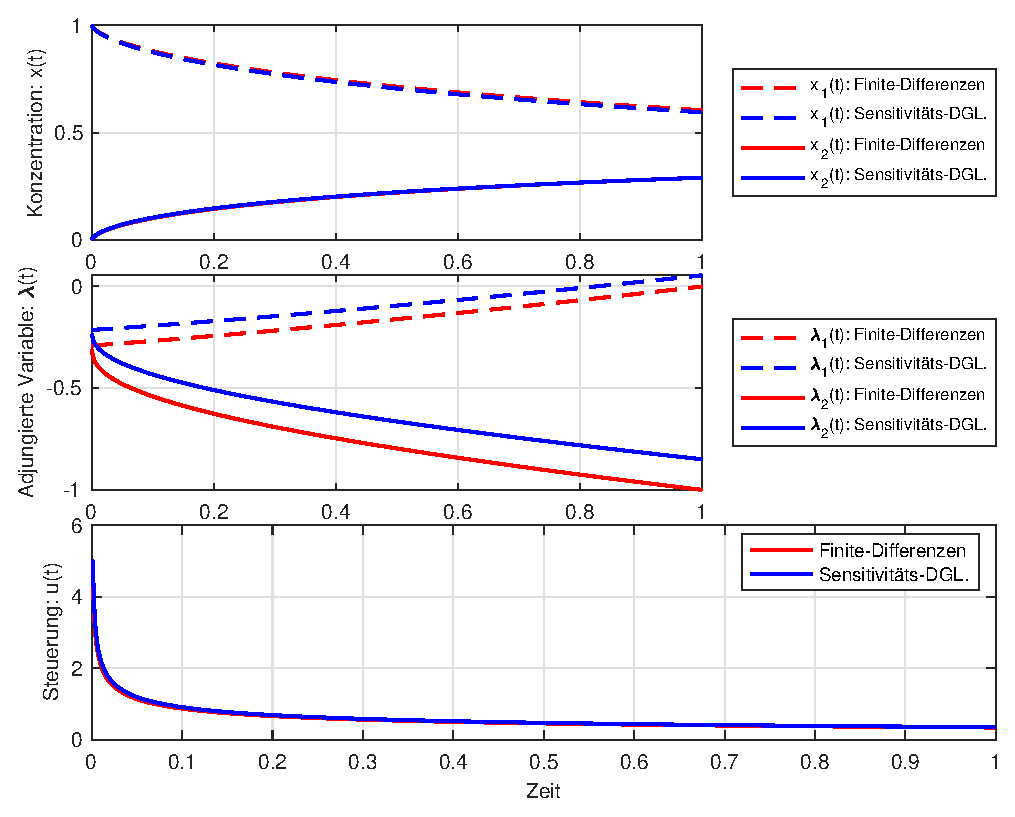
\includegraphics[width=.75\textwidth]{images/SingleShoot_Result}
	\caption{Indirektes Verfahren: Einfachschießverfahren}
	\label{fig:Einfach}
\end{figure}
Das Mehrfachschießverfahren, dargestellt in \autoref{fig:Mehrfach}, besitzt bei $N=10$ Stufen in der Lösung, welche die Stetigkeitsbedingungen an die Mehrzielknoten verletzen.\footnote{Hinweis: Zwischen den einzelnen Stufen gibt es keine Verbindungspunkte, Matlab interpoliert beim Plotten automatisch zwischen zwei Stufen.} Erst ab $N=25$ sind die Ergebnisse glatt und weisen keine Stufen mehr auf. Das Verhalten lässt sich mit einer ungünstigen Wahl der Startschätzung begründen. Die verwendete Implementierung des Mehrfachschießverfahrens nutzt zusätzlich für die globale Konvergenz des Newton-Schritts eine Armijo-Schrittweitensteuerung. Die Wahl der Startschätzung der Mehrzielknoten war für $N=10$ so ungünstig, dass die Armijo-Regel für eine der folgenden Iterationen keine Schrittweite im Rahmen der Maschinengenauigkeit gefunden hat, welche einen hinreichenden Abstieg sicherstellen würde. Aus diesem Grund wird das Verfahren frühzeitig abgebrochen und erzeugt die Treppen innerhalb der Lösung. Diese Beobachtung lässt sich bestätigen, wenn ein anderer Startwert für $N=10$ gewählt wird, bei welchem die Schrittweitensteuerung die folgenden Newton-Schritte ausreichend dämpfen kann (vgl. \autoref{fig:CompareMehrfach}). 

\begin{figure}[h!]
	\centering
	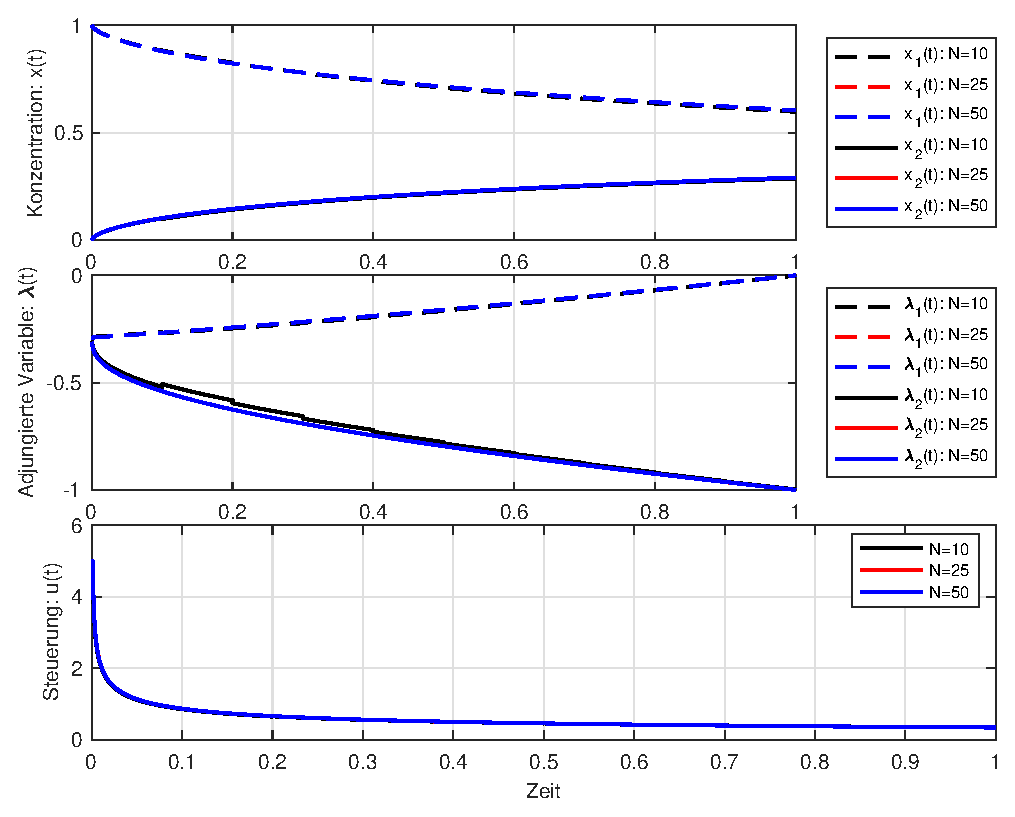
\includegraphics[width=.75\textwidth]{images/MultipleShoot_Result}
	\caption{Indirektes Verfahren: Mehrfachschießverfahren}
	\label{fig:Mehrfach}
\end{figure}


\begin{figure}[h!]
	\centering
	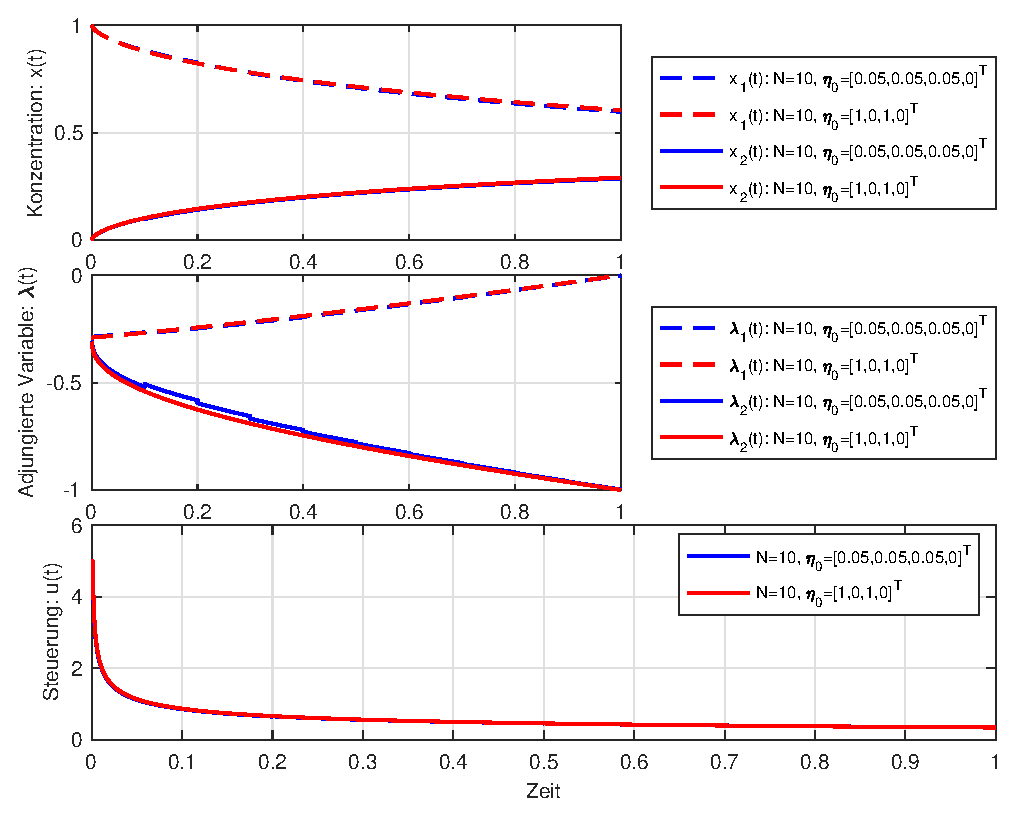
\includegraphics[width=.75\textwidth]{images/MultipleShoot_StartschaetzungVergleich_Result}
		\caption{Mehrfachschießverfahren ($N=10$): Vergleich verschiedener Startschätzungen}
	\label{fig:CompareMehrfach}
\end{figure}

Die stärkste Abhängigkeit von der Wahl der Startschätzung und Gitterpunktanzahl hat das Differenzenverfahren aufgezeigt, wobei die Startschätzung für aussagekräftige Lösungen bereits sehr nah an der Zieltrajektorie liegen musste. Zu diesen Zweck wurde das Ergebnis eines direkten Verfahrens aus \autoref{ch:DirectMehtods} für die Initialisierung der Startschätzung genutzt. Das Differenzenverfahren beruht auf der Lösung eines nichtlinearen Gleichungssystems. Der entsprechende Löser findet für $N=25$ keine Lösung. Ab $N\geq50$ sind die Ergebnisse sehr ähnlich und decken sich auch mit den vorherigen Lösungen der anderen Verfahren (vgl. \autoref{fig:Diff}).

\begin{figure}[h!]
	\centering
	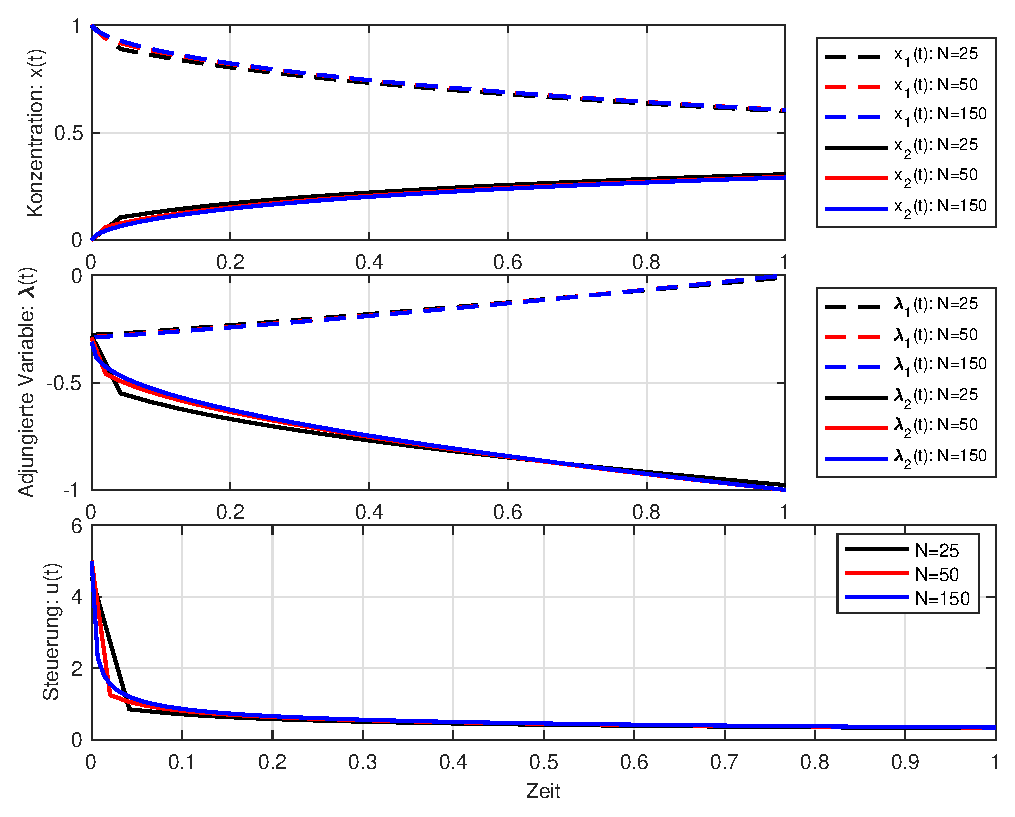
\includegraphics[width=.85\textwidth]{images/FiniteDiff_Result}
	\caption{Indirektes Verfahren: Differenzenverfahren}
	\label{fig:Diff}
\end{figure}

Das Matlab-Verfahren \textit{bvp4c} zur Lösung von Randwertproblemen nutzt die dreistufige Kollokationsformel \textit{Lobatto-IIIA} in Kombination mit einer Finiten-Differenzen-Implementierung.  \cite{bvp4c} Es besitzt für jede betrachtete Anzahl von Mehrzielknoten nahezu identische Lösungen (vgl. \autoref{fig:bvp4c}), weshalb eine Erhöhung der Anzahl keine erhebliche Auswirkung auf das Ergebnis aufzeigt. Ein möglicher Grund ist die von Matlab auf das Verfahren abgestimmte Ermittlung der Startschätzung.

\begin{figure}[h!]
	\centering
	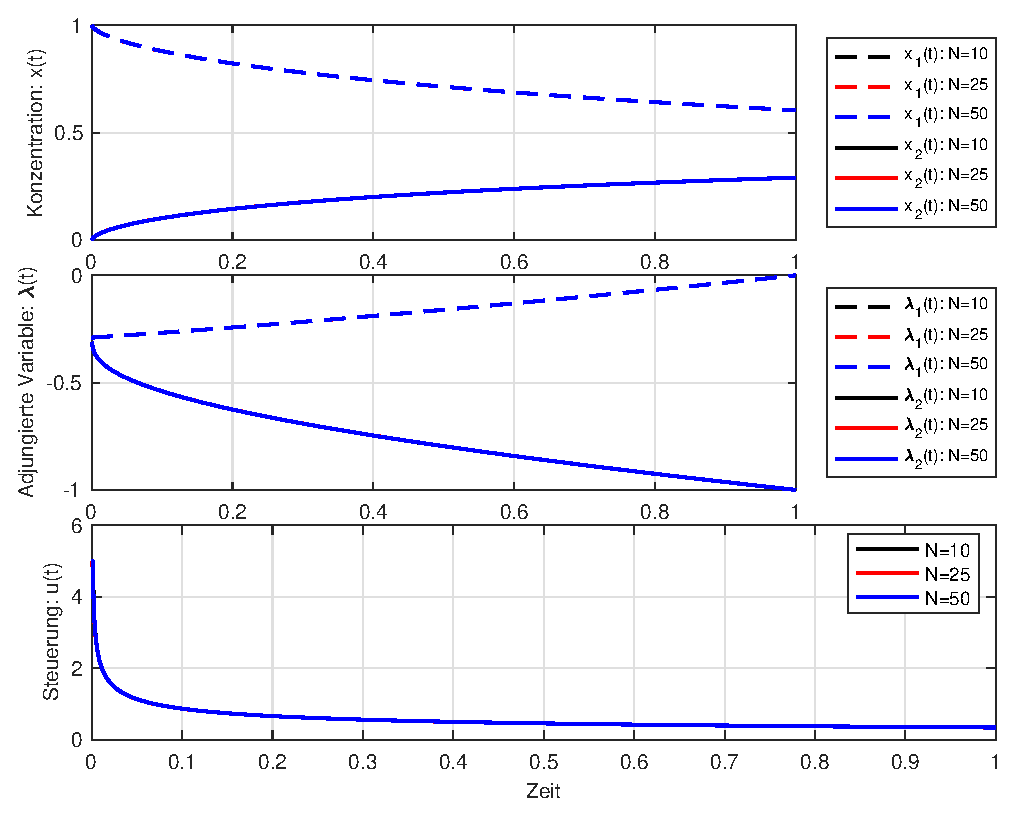
\includegraphics[width=.85\textwidth]{images/Matlab_bvp4c_Result}
	\caption{Indirektes Verfahren: bvp4c (Matlab-Verfahren)}
	\label{fig:bvp4c}
\end{figure}
\pagebreak
Alles in allem zeigt sich, dass wie bei den direkten Verfahren, grundsätzlich alle untersuchten Methoden unter gewissen Voraussetzungen eine sinnvolle Lösung berechnen und deshalb bei Gegenüberstellung in \autoref{fig:CompareBound} kaum zu unterscheiden sind. Die Konzentration von $x_1(t)$ wird kontinuierlich abgebaut und die von $x_2(t)$ gleichmäßig erhöht. Die Steuerung stabilisiert sich im Laufe der Zeit. Des Weiteren wird in \autoref{fig:CompareBound} ersichtlich, dass die Annahme (\ref{eq:anforderung_lambda2<lambda1_t>0}), welche besagt  $\lambda_1 > \lambda_2$, überall erfüllt ist. Durch $\lambda_2(t) < 0, \forall t \in [0,1]$ gilt sogar immer die strengere Eigenschaft $\lambda_1 > 3\lambda_2$, weshalb die Hamilton-Funktion immer ein globales Minimum für $u(t) \in \mathbb{R}, t \in (0,T]$ besitzt .

\begin{figure}[h!]
	\centering
	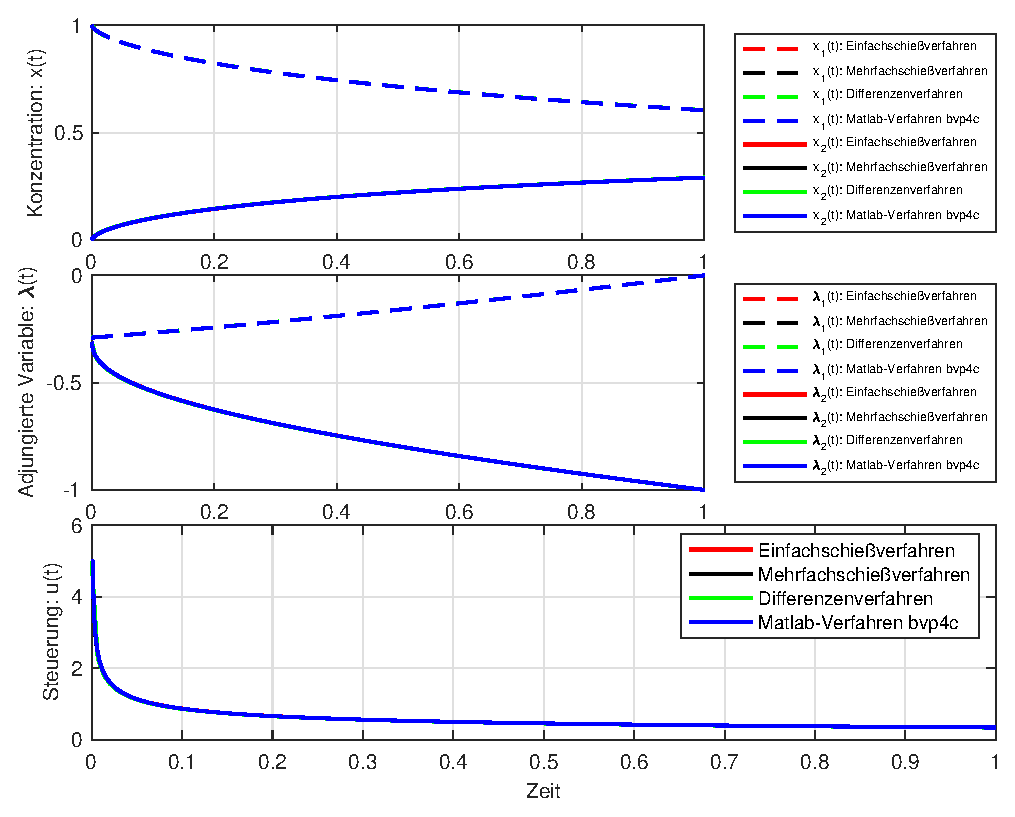
\includegraphics[width=1\textwidth]{images/CompareIndirect_Method}
	\caption{Indirekte Verfahren: Vergleich}
	\label{fig:CompareBound}
\end{figure}
%%%%%%%%%%%%%%%%%%%%%%%%%%%%%%%%%%%%%%%%%
%%%% Start Uncommetn
%\pagebreak
%
%
%\section{Temperaturverlauf}
%
%\begin{align}
%	u(t) &= k_1 = \exp\left(\frac{-\alpha}{\vartheta(t)}\right)			&&|\  \ln() \\
%	\ln(u(t)) &= \frac{-\alpha}{\vartheta(t)}												&&|\  \cdot \vartheta(t) \\
%	\ln(u(t)) \cdot \vartheta(t)&= -\alpha														&&|\  :  \ln(u(t)) \\
%	\vartheta(t)&= \frac{-\alpha}{\ln(u(t))}
%\end{align}

%\pagebreak
%
%\chapter{To-Do}
%\section{Offene Fragen}
%\begin{itemize}
%	\item $u=0$ darf gar nicht angenommen werden? $\Rightarrow$ Ausschließbar über die Definition? Oder nicht ausschließbar?
%	\item Vorgegebene Definition/ Form der Steuerfunktion schließt Fälle für $u \leq 0$  aus, wie behandeln wir diese? $\Rightarrow$ Ausdruck $h$ kann in der Theorie kleiner gleich Null werden 
%	\item Richtige Formulierung des Randwertproblem/ Braucht man bei der Fallunterscheidung eine explizite Abhängigkeit von der Zeit?
%	\item Muss die Stetigkeit der Steuerfunktion nachgewiesen werden bzw. wie weist man die in unserem Fall nach, um Pontryagin anwenden zu können? $\Rightarrow$ Satz von Weierstraß? $\Rightarrow$ Im Intervall gibt es immer ein eindeutiges Minimum $\Rightarrow$ Reicht das als Regularitätsnachweis bzw. als Stetigkeitsnachweis für Pontryagin?
%	\item Ist Grenzbetrachtung für $t=0$ richtiger Ansatz um den Fall $x_2(0) =0$ zu betrachten? $\Rightarrow$ Ist eigentlich ein Sattelpunkt, da dann $H_{uu} = 0$ und somit mit in der Fallunterscheidung abgedeckt
%\end{itemize}
%
%<<<<<<< HEAD
%\pagebreak
%
%\section{Keine eindeutige Extremstelle}
%Im Weiteren sei:
%\begin{itemize}
%	\item  $\lambda_1 > \lambda_2$
%	\item $x_1(t) > 0 \forall t \in [0,1]$ und 
%	\item $x_2(t)>0 \forall t \in (0,T]$
%\end{itemize}
%vorausgesetzt. Wird die partielle Ableitung  ($H_u$) der Hamilton-Funktion nach $u$ näher betrachtet, fällt auf, dass für $x_2(0) = 0$ und für $\lambda_1 = 3\lambda_2$ \textcolor{red}{über die analytische Betrachtung} von $H_u$ und $H_{uu}$ keine eindeutige Extremstelle gefunden werden kann. Aus diesem Grund betrachten wir im weiteren beide Fälle einzeln:
%
%=======
%\section{Keine eindeutige Extremstelle}
%Im Weiteren sei:
%\begin{itemize}
%	\item  $\lambda_1 > \lambda_2$
%	\item $x_1(t) > 0 \forall t \in [0,1]$ und 
%	\item $x_2(t)>0 \forall t \in (0,T]$
%\end{itemize}
%vorausgesetzt. Wird die partielle Ableitung  ($H_u$) der Hamilton-Funktion nach $u$ näher betrachtet, fällt auf, dass für $x_2(0) = 0$ und für $\lambda_1 = 3\lambda_2$ \textcolor{red}{über die analytische Betrachtung} von $H_u$ und $H_{uu}$ keine eindeutige Extremstelle gefunden werden kann. Aus diesem Grund betrachten wir im weiteren beide Fälle einzeln:
%
%>>>>>>> joshua
%\textbf{1. Fall: $x_2(0) = 0$}
%\\Dieser Fall tritt nur im Startpunkt auf, da die Konzentration aus physikalischer Sicht nicht negativ werden kann und $x_2(T)$ zu maximieren ist. Im Startpunkt gilt:
%\begin{align}
%		H(t,x,\lambda,u) =&  - \lambda_1 u x_1(t)+  \lambda_1 u^2x_2(t)  +  \lambda_2  u x_1(t) -  3 \lambda_2 u^2x_2(t)\\
%		H(0,[1,0]^T,\lambda,u) =&  - \lambda_1 u +  \lambda_2  u\\
%		&\nonumber\\
%		H_u(t,x,\lambda,u)  =&  - \lambda_1  x_1(t)+  2 \lambda_1 u x_2(t)  +  \lambda_2  x_1(t) -  6 \lambda_2  u x_2(t)\\
%		H_u(0,[1,0]^T,\lambda,u)  =&  - \lambda_1 +  \lambda_2
%\end{align}
%Durch die Voraussetzung von $\lambda_1 > \lambda_2$ ist somit im Punkt $t=0$ zu beobachten, dass die Schaltfunktion $H_u < 0$ ist, unabhängig von $u$. Die Hamilton-Funktion weist dadurch im Punkt $t=0$ immer eine negative Steigung auf. Aus diesem Grund wird ein eindeutiges Minimum auf dem rechten Rand für $u(0)=5$ angenommen:
%\begin{align}
%	H(0,[1,0]^T,\lambda,u) =&  - \lambda_1 u +  \lambda_2  u = \underbrace{(- \lambda_1+ \lambda_2)}_{<0} \cdot u 
%\end{align}
%<<<<<<< HEAD
%=======
%
%\textbf{2. Fall: $\lambda_1 = 3\lambda_2$}
%\\Auch in diesem Fall wird $x_1(t) > 0$ und $\lambda_1 > \lambda_2$ angenommen, wodurch auch hier: $H_u =  \lambda_2 -  \lambda_1 < 0$ folgt. Äquivalent zum 1. Fall nimmt die Hamilton-Funktion wieder das eindeutige Minimum auf dem rechten Rand $u(t)=5$ an, da gilt:
%\begin{align}
%	\arg \min_{u \in [0,5]} (- \lambda_1+ \lambda_2)\cdot u = 5
%\end{align}
%>>>>>>> joshua
%
%\textbf{2. Fall: $\lambda_1 = 3\lambda_2$}
%\\Auch in diesem Fall wird $x_1(t) > 0$ und $\lambda_1 > \lambda_2$ angenommen, wodurch auch hier: $H_u =  \lambda_2 -  \lambda_1 < 0$ folgt. Äquivalent zum 1. Fall nimmt die Hamilton-Funktion wieder das eindeutige Minimum auf dem rechten Rand $u(t)=5$ an, da gilt:
%\begin{align}
%	\arg \min_{u \in [0,5]} (- \lambda_1+ \lambda_2)\cdot u = 5
%\end{align}

%\begin{itemize}
%	\item Was passiert bei $t=0$, da  dort $x_2(0) = 0 $, somit bereits gefundenes $u$ nicht definiert und $u^* \overset{!}{>} 0$. Intuitiver Ansatz es einfach auf $u_{min}=0$ zu setzen funktioniert nicht!
%	\item Was passiert mit Bedingung an $\lambda \rightarrow$ von $H_{uu}$? 
%	\item Fallunterscheidung auf $t$ zurückführen
%	\item Hinweise Jörn
%\end{itemize}


%
%
%
%
%Im nächsten Schritt wird überprüft, ob das Minimum im Inneren der Steuerbeschränkung angenommen wird, d.h. ob $u^* \in \overset{\circ}{U} = (0,5)$.  Zu diesem Zweck wird \autoref{eq:Steuerfunktion} unter der Bedingung $\lambda_1 > 3\lambda_2$  näher analysiert.
%\begin{align}
%	u  &= \frac{(\lambda_1-\lambda_2) \cdot  x_1(t)}{(2 \lambda_1 -  6 \lambda_2) \cdot  x_2(t)}\\
%		&= \left[\frac{\lambda_1}{2 \lambda_1 -  6 \lambda_2} - \frac{\lambda_2}{2 \lambda_1 -  6 \lambda_2}\right]\cdot \frac{x_1(t)}{x_2(t)}\\
%		&= \left[\frac{1}{2 -  2 \underbrace{\frac{3\lambda_2}{\lambda_1}}_{< 1}} - \frac{1}{2 \underbrace{\frac{\lambda_1}{\lambda_2}}_{>1} -  6 }\right]\cdot \frac{x_1(t)}{x_2(t)}
%\end{align}
%
%
%
%
%
%\pagebreak
%
%
%
%
%
%
%\begin{align}
%	H(t,x,\lambda,u) &= - \lambda_1 u x_1(t)+  \lambda_1 u^2x_2(t)  +  \lambda_2  u x_1(t) -  3 \lambda_2 u^2x_2(t)\\
%										&= - \underbrace{\left[\lambda_1  x_1(t) - \lambda_2  x_1(t)\right]}_{=:\phi(t)} \cdot u + \underbrace{\left[\lambda_1 x_2(t) -  3 \lambda_2 x_2(t)\right]}_{=:\gamma(t)}\cdot u^2\\
%										&= -\phi(t) u + \gamma(t) u^2
%\end{align}
%Setzt man nun die berechnet Steuerfunktion
%\begin{align}
%	u  = \frac{\lambda_1(t)  x_1(t)-\lambda_2(t)  x_1(t)}{2 \lambda_1(t) x_2(t) -  6 \lambda_2(t)  x_2(t)} = \frac{\phi(t) }{2 \gamma(t)}
%\end{align}
%in die Hamilton-Funktion ein und nutzt aus, dass ein autonomes System vorliegt, folgt:
%\begin{align}
%	H(t,x,\lambda,u) &= -\phi(t) u + \gamma(t) u^2 =  -\phi(t) \cdot \left[\frac{\phi(t) }{2 \gamma(t)}\right] + \gamma(t) \cdot \left[\frac{\phi(t) }{2 \gamma(t)}\right]^2\\[10pt]
%	&= \frac{-\phi(t)^2 }{2 \gamma(t)} + \frac{\phi(t)^2}{4 \gamma(t)} = \frac{-2\phi(t)^2 }{4 \gamma(t)} + \frac{\phi(t)^2}{4 \gamma(t)}=  \frac{-\phi(t)^2}{4 \gamma(t)}\\[10pt]
%	 &= \frac{\phi(t)}{2\gamma(t)} \cdot \frac{- \phi(t)}{2} = u \cdot \frac{- \phi(t)}{2}\\[10pt]
%	%&= \frac{-\left[\lambda_1  x_1(t) - \lambda_2  x_1(t)\right]^2}{4 \cdot \left[\lambda_1 x_2(t) -  3 \lambda_2 x_2(t)\right]}
%\end{align}
%
%Wir wissen, Hamilton-Funktion ist konstant über den gesamten Intervall. Betrachte deshalb zwei unterschiedliche Punkte $t=0$ und $t=T=1$:
%\begin{align}
%	\phi(0)  =& \lambda_1(0)  x_1(0)-\lambda_2(0)  x_1(0) &&= \lambda_1(0)  -\lambda_2(0) \\
%	\phi(T) =& \lambda_1(T)  x_1(T)-\lambda_2(T)  x_1(T) &&= x_1(T)\\
%	\gamma(0) =& 2 \lambda_1(0) x_2(0) -  6 \lambda_2(0)  x_2(0) &&= 0\\
%	\gamma(T) =& 2 \lambda_1(T) x_2(T) -  6 \lambda_2(T)  x_2(T) &&= 6  x_2(T)
%\end{align}
%
%Daraus folgt:
%\begin{align}
%		H(0,x(0),\lambda(0),u(0))=&  \frac{-\phi(0)^2}{4 \gamma(0)}\\
%		H(T,x(T),\lambda(T),u(T))=&  \frac{-\phi(T)^2}{4 \gamma(T)}
%\end{align}


%\begin{align}
%	H(0,x_0,\lambda(0),u(0))     =& - \left[\lambda_1(0)  x_1(0) - \lambda_2(0)  x_1(0)\right] \cdot u(0) + \nonumber \\
%	&\left[\lambda_1(0) x_2(0) -  3 \lambda_2(0) x_2(0)\right]\cdot u(0)^2\\
%	=& - \left[\lambda_1(0) - \lambda_2(0) \right] \cdot u(0)
%\end{align}
%Für $t=T=1$ gilt $\lambda(T) = (0,-1)^T$ und somit:
%\begin{align}
%	H(T,x(T),\lambda(T),u(T)) =& - \left[\lambda_1(T)  x_1(T) - \lambda_2(T)  x_1(T)\right] \cdot u(T) + \nonumber\\
%	&\left[\lambda_1(T) x_2(T) -  3 \lambda_2(T) x_2(T)\right]\cdot u(T)^2\\
%	=& -  x_1(T)  \cdot u(T) + 3 x_2(T) \cdot u(T)^2
%\end{align}
